\documentclass[12pt,t]{beamer}

%------------------------------------------------------------------------------
% configuration
%------------------------------------------------------------------------------
\RequirePackage{etex}
\usepackage{../../themes/dbt}
\usepackage{catchfilebetweentags}

\setbeameroption{hide notes}
\setbeamertemplate{caption}{\raggedright\insertcaption\par}

\graphicspath{{images/}}

% a few macros
\newcommand{\bi}{\begin{itemize}}
\newcommand{\ei}{\end{itemize}}
\newcommand{\ig}{\includegraphics}
\newcommand{\myhref}[1]{\href{#1}{\tt \scriptsize #1}}
\newcommand{\incnote}[1]{\note{\ExecuteMetaData[notes.tex]{#1}}}
\newcommand{\src}[2]{\vspace{-10pt}\caption{\href{#1}{\centering \tt \tiny [#2]}}}

%------------------------------------------------------------------------------
% title
%------------------------------------------------------------------------------
% slide
\title{Systèmes d'exploitation pour l'embarqué}
\subtitle{UV 5.2 - Exécution et Concurrence}

\author{\href{}{Paul Blottière}}
\institute{
    \href{http://www.ensta-bretagne.fr/}{ENSTA Bretagne} \\[2pt]
    \href{}{\tt \scriptsize 24 Novembre 2015}
}
\date{
    \href{https://github.com/pblottiere}{\tt \scriptsize https://github.com/pblottiere} \\[2pt]
    %\href{blottiere.paul@gmail.com}{\tt \scriptsize blottiere.paul@gmail.com}
}

% info
\begin{document}

{
\setbeamertemplate{footline}{} % no page number here
\frame{
    \titlepage
    \incnote{title}
} }

%------------------------------------------------------------------------------
% amélioration continue
%------------------------------------------------------------------------------
\begin{frame}{Amélioration continue}
    \subt{Contributions}
    \vspace{12pt}

    \begin{center}
    
\includegraphics[scale=0.7]{github.png}
    \end{center}

    \bi
    \itemsep12pt
    \item Dépôt du cours : \href{https://github.com/pblottiere/embsys}{\tt \scriptsize https://github.com/pblottiere/embsys}

    \onslide<2->{
        \item Souhaits d'amélioration, erreurs, idées de TP, ... : ouverture d'Issues (avec le bon label!)
        \item Apports de corrections : Pull Request
        \ei
    }
\end{frame}

%<**lecture_content>
%------------------------------------------------------------------------------
% lecture
%------------------------------------------------------------------------------
\begin{frame}[plain,c]
    \centering
    \huge\textcolor{title}{IPC et programmation réseau}
\end{frame}

%------------------------------------------------------------------------------
% plan
%------------------------------------------------------------------------------
\begin{frame}{Plan}
    \subt{}
    \vspace{10pt}

    \begin{enumerate}
        \itemsep12pt
        \item Descripteur de fichier
        \item IPC : qu'est-ce?
        \item Pipe
        \item File de message
        \item Mémoire partagée
        \item Sémaphore
        \item Les sockets
        \item Multiplexage d'entrées / sorties
    \end{enumerate}

    \note {
    }
\end{frame}

%------------------------------------------------------------------------------
% fd1
%------------------------------------------------------------------------------
\begin{frame}{Descripteur de fichier (1)}
    \subt{Généralités}
    \vspace{15pt}

    File descriptor : entier compris entre 0 et OPEN\_MAX.

    \onslide<2->{
        \vspace{15pt}
        Trois descripteurs réservés :
        \bi
        \itemsep6pt
        \item 0 : STDIN\_FILENO
        \item 1 : STDOUT\_FILENO
        \item 2 : STDERR\_FILENO
        \ei
    }

    \onslide<3->{
        \vspace{15pt}
        Un flux de type {\textbf{FILE *}} est associé aux descripteurs de fichier
        par défaut :
        \bi
        \itemsep6pt
        \item stdin
        \item stdout
        \item stderr
        \ei
    }

    \incnote{fd1}
\end{frame}

%------------------------------------------------------------------------------
% fd2
%------------------------------------------------------------------------------
\begin{frame}{Descripteur de fichier (2)}
    \subt{/proc/<PID>/fd/}

    \vspace{20pt}
    Une liste de tous les file descriptor d'un processus est disponible dans
    le {\textbf{/proc}} :

    \vspace{15pt}
    \begin{figure}
        \centering
        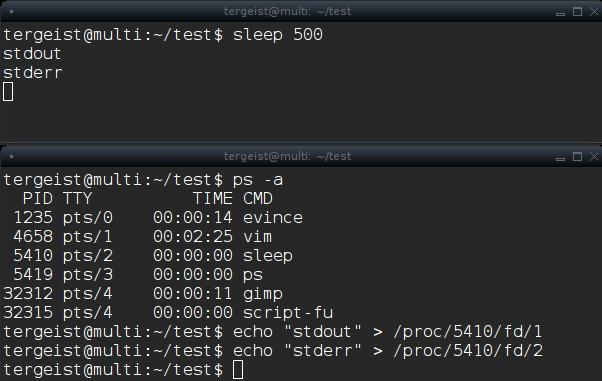
\includegraphics[scale=0.7]{fd_proc.png}
    \end{figure}

\end{frame}

%------------------------------------------------------------------------------
% ipc1
%------------------------------------------------------------------------------
\begin{frame}{IPC : qu'est-ce?}
    \subt{Définition}

    \vspace{15pt}
    Entres threads, la communication est simple : données partagées au sein
    du même espace mémoire.

    \onslide<2->{
        \vspace{15pt}
        Dans le cas de communication entre processus, des mécanismes sont
        nécessaires!
    }

    \onslide<2->{
        \vspace{15pt}
        Ce sont les Inter Process Communication (définis par SUSv4) :
        \bi
        \itemsep12pt
        \item pipe
        \item file de messages
        \item mémoire partagée (et sémaphore pour la synchronisation)
        \ei
    }

\end{frame}

%------------------------------------------------------------------------------
% pipe1
%------------------------------------------------------------------------------
\begin{frame}{Pipe (1)}
    \subt{Principe}

    \vspace{10pt}
    Moyen de communication unidirectionnel.

    \onslide<2->{
        \vspace{10pt}
        Deux extrémités représentées par des file descriptor :
        \vspace{8pt}
        \begin{figure}
            \centering
            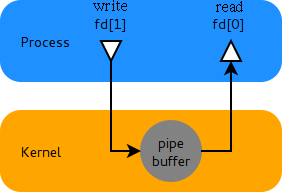
\includegraphics[scale=0.6]{pipe.png}
            \src{http://hzqtc.github.io/2012/07/linux-ipc-with-pipes.html}{Pipe}
        \end{figure}
    }

    \vspace{-5pt}
    \onslide<3->{
        => comme les fd doivent être connus pour l'écriture  et la lecture, les
        pipe sont utilisables avec les threads ou les processus dupliqués (fork)!
    }

\end{frame}

%------------------------------------------------------------------------------
% pipe2
%------------------------------------------------------------------------------
\begin{frame}[fragile]{Pipe (2)}
    \subt{Comment?}

    \vspace{15pt}
    Cinq fonctions :
    \vspace{8pt}
    \bi
    \itemsep12pt
    \item {\textbf{pipe}} : création du tube
    \item {\textbf{write}} : écriture dans le tube
    \item {\textbf{read}} : lecture des données
    \item {\textbf{close}} : fermeture du tube
    \ei

    \vspace{15pt}
    \begin{lstlisting}
#include <unistd.h>

pipe(int pipefd[2]);
    \end{lstlisting}

\end{frame}

%------------------------------------------------------------------------------
% pipe3
%------------------------------------------------------------------------------
\begin{frame}{Pipe (3)}
    \subt{pipe.c}

    TODO

\end{frame}

%------------------------------------------------------------------------------
% pipe4
%------------------------------------------------------------------------------
\begin{frame}{Pipe (4)}
    \subt{Named pipe}

    \vspace{15pt}
    Pour faire communiquer des processus distincts (n'ayant pas accès au file
    descriptor du tube), il existe des {\textbf{tube nommé}}.

    \onslide<2->{
        \vspace{15pt}
        Contrairement au tube simple résidant en mémoire, un tube nommé possède une
        représentation au sein du système de fichier.

        \vspace{5pt}
        \begin{figure}
            \centering
            
\includegraphics[scale=0.17]{tux_pipe.png}
        \end{figure}
    }

\end{frame}

%------------------------------------------------------------------------------
% pipe5
%------------------------------------------------------------------------------
\begin{frame}[fragile]{Pipe (5)}
    \subt{Named pipe}

    \vspace{10pt}
    Six fonctions :
    \vspace{5pt}
    \bi
    \itemsep6pt
    \item {\textbf{mkfifo}} : création dy fichier représentant le tube
    \item {\textbf{open}} : ouverture du tube
    \item {\textbf{write}} : écriture de données dans le tube
    \item {\textbf{read}} : lecture des données
    \item {\textbf{close}} : fermeture du tube
    \item {\textbf{unlink}} : suppression du fichier représentant le tube
    \ei

    \vspace{15pt}
    \begin{lstlisting}
#include <sys/stat.h>

int mkfifo(const char * pipe_name, mode_t mode);
    \end{lstlisting}

\end{frame}

%------------------------------------------------------------------------------
% pipe6
%------------------------------------------------------------------------------
\begin{frame}{Pipe (6)}
    \subt{named\_pipe.c}

    TODO
\end{frame}

%------------------------------------------------------------------------------
% msg1
%------------------------------------------------------------------------------
\begin{frame}{File de messages (1)}
    \subt{Différence avec les tubes}

    \vspace{15pt}
    La communication par tubes se fait par l'intermédiaire de flux : la taille
    des données peut être variable entre chaque écriture/lecture.

    \onslide<2->{
        \vspace{15pt}
        La communication par file de message se fait par passage de message de
        taille fixe avec des niveaux de priorité!

        \vspace{15pt}
        \begin{figure}
            \centering
            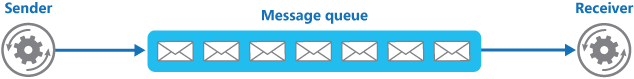
\includegraphics[scale=0.5]{msgq.png}
            \src{https://msdn.microsoft.com/en-us/library/dn589781.aspx}{Message Queue}
        \end{figure}
    }

    \incnote{msg1}

\end{frame}

%------------------------------------------------------------------------------
% msg2
%------------------------------------------------------------------------------
\begin{frame}[fragile]{File de message (2)}
    \subt{Comment?}

    \vspace{10pt}
    Les 5 appels système principaux :
    \vspace{5pt}
    \bi
    \itemsep8pt
    \item {\textbf{mq\_open}} : ouverture d'une file
    \item {\textbf{mq\_close}} : fermeture de la file
    \item {\textbf{mq\_unlink}} : destruction de la file
    \item {\textbf{mq\_send}} : envoie d'un message dans la file
    \item {\textbf{mq\_receive}} : réception d'un message
    \ei

    \vspace{10pt}
    \begin{lstlisting}
#include <mqueue.h>

mqd_t mq_send(mqd_t mq, const char * msg,
              size_t size_msg,
              unsigned int priority);
    \end{lstlisting}

\end{frame}

%------------------------------------------------------------------------------
% msg3
%------------------------------------------------------------------------------
\begin{frame}{File de message (3)}
    \subt{mq.c}

    TODO
\end{frame}

%------------------------------------------------------------------------------
% shm1
%------------------------------------------------------------------------------
\begin{frame}{Mémoire partagée (1)}
    \subt{Principe}

    \vspace{10pt}
    Shared memory : segment de mémoire accessible en lecture / écriture par
    plusieurs processus et persistant jusqu'au {\textbf{reboot}} de la
    machine.

    \vspace{15pt}
    \begin{figure}
        \centering
        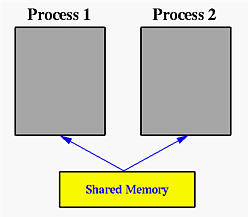
\includegraphics[scale=0.5]{shm.jpg}
        \src{http://www.csl.mtu.edu/cs4411.ck/www/NOTES/process/shm/what-is-shm.html}{Shared memory}
    \end{figure}

\end{frame}

%------------------------------------------------------------------------------
% shm2
%------------------------------------------------------------------------------
\begin{frame}[fragile]{Mémoire partagée (2)}
    \subt{Les appels système}

    \vspace{15pt}
    Quatre appels système :
    \vspace{5pt}
    \bi
    \itemsep8pt
    \item {\textbf{shm\_open}} : ouverture du segment mémoire
    \item {\textbf{ftruncate}} : dimensionnement du segment
    \item {\textbf{mmap}} : projection de la srtucture de donnée sur le segment
    \item {\textbf{shm\_unlink}} : destruction du segment
    \ei

    \vspace{10pt}
    \begin{lstlisting}
int shm_open(const char * name, int flags,
             mode_t mode);
    \end{lstlisting}

\end{frame}

%------------------------------------------------------------------------------
% shm3
%------------------------------------------------------------------------------
\begin{frame}{Mémoire partagée (3)}
    \subt{shm.c}
\end{frame}

%------------------------------------------------------------------------------
% sem1
%------------------------------------------------------------------------------
\begin{frame}{Sémaphore (1)}
    \subt{Principe}

    \vspace{15pt}
    Les communications multiprocessus à travers la mémoire partagée peut
    conduire à des incohérences dans les données si les accès ne sont pas
    synchronisés!

    \vspace{15pt}
    => contrôle d'accès aux ressources critiques via les sémaphores!

    \vspace{20pt}
    On peut aussi gérer le nombre d'accès simultané maximum autorisé!
\end{frame}

%------------------------------------------------------------------------------
% sem2
%------------------------------------------------------------------------------
\begin{frame}{Sémaphore (2)}
    \subt{flags levés / baissés}

    \vspace{12pt}
    L'accès à la donnée :
    \vspace{5pt}
    \begin{enumerate}
        \itemsep8pt
        \item un processus attend que le flag soit levé (ressource disponible)
        \item le processus baisse le flag
        \item le processus utilise la ressource protégée
        \item le processus lève le flag pour indiquer qu'elle est disponible
        \item le kernel réveille les autres processus en attente
    \end{enumerate}
\end{frame}

%------------------------------------------------------------------------------
% sem3
%------------------------------------------------------------------------------
\begin{frame}[fragile]{Sémaphore (3)}
    \subt{versus mutex}

    \vspace{15pt}
    Mutex : surtout utilisé dans les applications multithreads (protection
    d'accès d'une section de code ne pouvant pas être exécutée par plus d'un
    thread).

    \vspace{15pt}
    Sémaphore : surtout utilisé pour les communications multiprocessus.

    \vspace{15pt}
    Mutex = Sémaphore local avec un nombre de clé de 1 (sémaphore binaire)

    \begin{lstlisting}
sem_init(&mutex, 0, 1);
    \end{lstlisting}
\end{frame}

%------------------------------------------------------------------------------
% sem3
%------------------------------------------------------------------------------
\begin{frame}{Sémaphore (3)}
    \subt{Sémaphore nommé}

\end{frame}

%------------------------------------------------------------------------------
% conclusion
%------------------------------------------------------------------------------
\begin{frame}{Conclusion}

    \centering
    \vspace{20pt}
    \LARGE{
    }

\end{frame}

%------------------------------------------------------------------------------
% ref
%------------------------------------------------------------------------------
\begin{frame}{Références}
    \vspace{30pt}

    \bi
    \itemsep12pt
    \item Linux Embarqué - Pierre Ficheux
    \item Développement système sous Linux - Christophe Blaess
    \item Modern Operating Systems - Andrew Tanenbaum
    \ei
\end{frame}
%<//lecture_content>

\end{document}
